\chapter{Articulation Work} % (fold)
\label{cha:articulation_work}

In diesem Kapitel wird das Konzept „Articulation Work“ dargestellt und in den Kontext von menschlicher Arbeit an sich gestellt. Der zweite Teil des Kapitels widmet sich den Aktivitäten, die „Articulation Work“ ausmachen, den Merkmalen, an denen sich gute „Articulation Work“ zeigt, sowie den Möglichkeiten der Unterstützung von „Articulation Work“ durch organisationale und technische Maßnahmen.

\section{Begriffsbestimmung} % (fold)
\label{sec:aw_begriffsbestimmung}

Das Konzept der "Articulation Work" wurde als Erklärungsmodell für einen bestimmten Typus von menschlicher Arbeit Mitte der 1980er Jahre von  \citet{Strauss85} im Kontext von Fallstudien aus der Krankenhaus-Organisation eingeführt. "Articulation Work" ist dabei jener Anteil an menschlicher Arbeit, der der Abstimmung mit anderen Individuen dient. Diese Abstimmung ist notwendig um das eigentliche Arbeitsziel erreichen zu können. Arbeit wird als inhärent kooperative Prozess gesehen, der immer auf Interaktion mit anderen Menschen basiert bzw. diese bedingt (Strauss formuliert diese Annahme in Bezugnahme auf \citet{Hughes71} prägnant mit der Aussage \emph{„work rests ultimately on interaction“}). Diese Annahme erscheint insofern als zulässig, als dass selbst Arbeitsabläufe, die selbst keine Kooperation mit anderen Menschen bedingen, zumindest auf den Ergebnissen anderer Arbeitsabläufe aufbauen oder als Grundlage weiterer Arbeitsabläufe dienen. Interaktion tritt also in jedem Arbeitsprozess zumindest zu Beginn und am Ende in unmittelbarer oder mittelbarer\footnote{Unter "mittelbar" ist hier Interaktion zu verstehen, die nicht im direkten Kontakt zwischen Individuen abläuft sondern lediglich indirekt durch die Ergebnisse eines Arbeitsprozesses (Materialien, Dokumente, \ldots) vermittelt wird.} Form auf.

\textbf{Abbildung, in der kooperative Arbeitsprozesse und solche mit mittelbarer und unmittelbarer Interaktion zu Beginn oder am Ende dargestellt werden}

Jener Teil von Arbeit, der der eigentlichen Zielerreichung dient, wird im hier vorgestellten Erklärungsmodell als „Production Work“ bezeichnet \citep{Fujimura87}. „Production Work“ ist komplementär zu „Articulation Work“ zu sehen und umfasst alle Aktivitäten, die der „Wertschöpfung“ im wörtlichen Sinn, also der Schaffung jener Werte (oder Ergebnisse), die durch den Arbeitsablauf erreicht werden sollten. Wenn hier von Arbeit bzw. Arbeitsabläufen die Rede ist, so ist darunter eine Kette von Aktivitäten zu verstehen, die der Erreichung eine vorab gewählten Ziels dient\footnote{siehe dazu etwa die Definition von Arbeit durch \citet{Semmer04}: \emph{„Arbeit ist zielgerichtete menschliche Tätigkeit zum Zwecke der Transformation und Aneignung der Umwelt aufgrund selbst- oder fremddefinierter Aufgaben, mit gesellschaftlicher, materieller oder ideeller Bewertung, zur Realisierung oder Weiterentwicklung individueller oder kollektiver Bedürfnisse, Ansprüche und Kompetenzen.“}}. 

\begin{figure}[htbp]
	\centering
		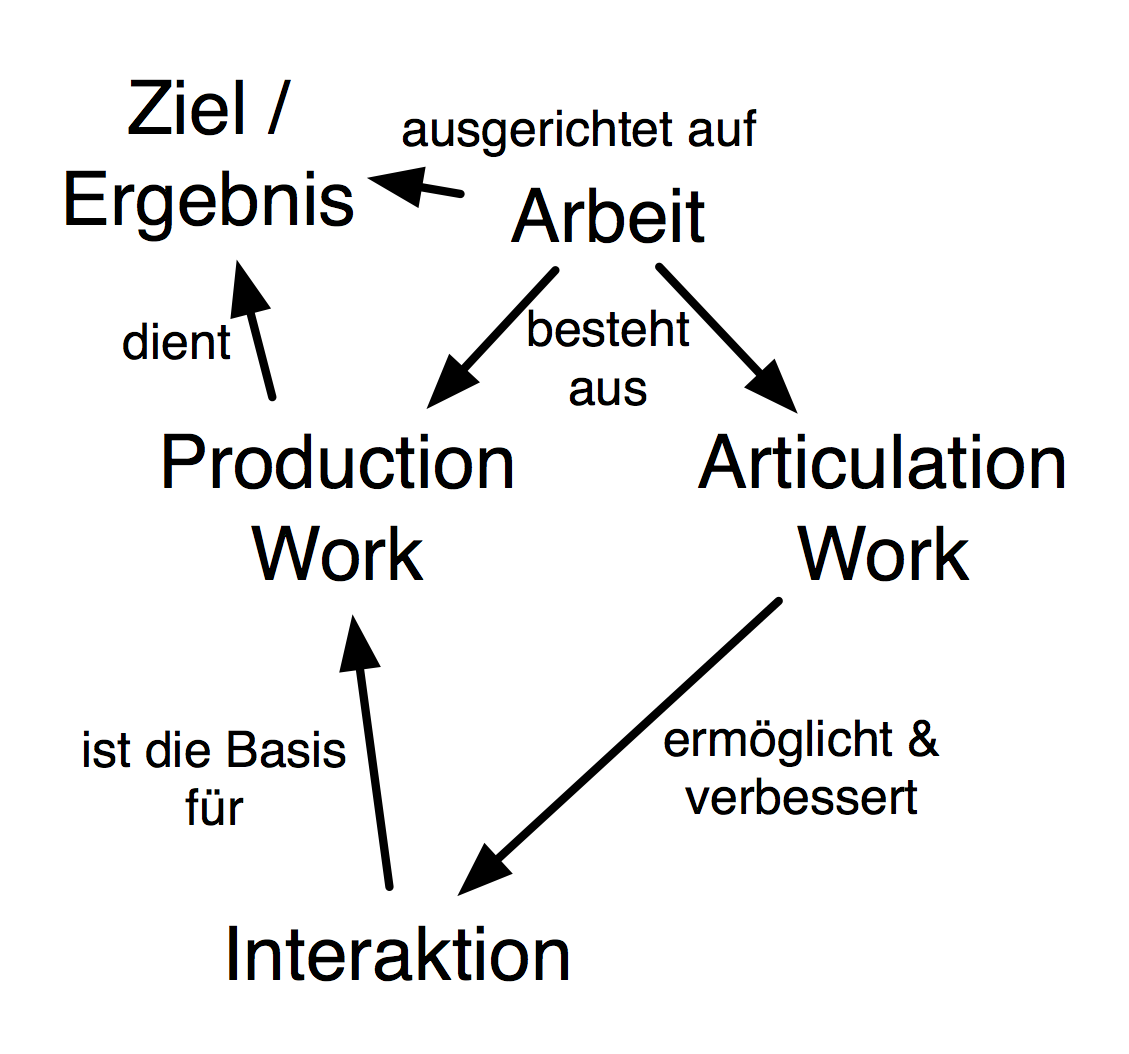
\includegraphics[height=3in]{img/ArticulationWork/ArbeitInteraktion.png}
	\caption{Struktur von Arbeitsabläufen}
	\label{fig:img_ArticulationWork_ArbeitInteraktion}
\end{figure}

Teile eines Arbeitsablaufs dienen also der Zielerreichung an sich („Production Work“). Andere Teile dienen der Abstimmung zwischen den involvierten Akteuren, um ein gemeinsames Verständnis über die jeweiligen Schnittstellen – also die Berührungspunkte zwischen den Tätigkeiten – zu entwickeln. Diese „Koordination“ ist kritisch für den Erfolg von kooperativer Arbeit \citep{Strauss93} und wird als „Articulation Work“ bezeichnet.\footnote{\emph{„Without an understanding of articulation, the gap between requirements and the actual work process in the office will remain inaccessible to analysis. That is, it will be possible to describe tasks in an idealized form but not to describe actual situations.“}\citep{Gerson86}} „Articulation Work“ ist damit ein Enabler für funktionierende Kommunikation und Koordination im eigentlichen Arbeitsprozess\footnote{\emph{"Reconciling incommensurate assumptions and procedures in the absence of enforceable standards is the essence of articulation. Articulation consists of all the tasks involved in assembling, scheduling, monitoring, and coordinating all of the steps necessary to complete a production task."}\citep{Gerson86}}. 

\begin{figure}[htbp]
	\centering
		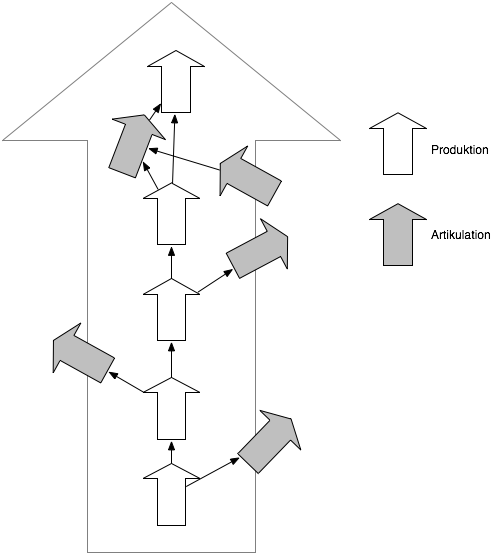
\includegraphics[height=3in]{img/ArticulationWork/ArtikulationProduktion.png}
	\caption{Konzeptualisierung von „Arbeit“ nach \citep{Strauss85} und \citep{Fujimura87}}
	\label{fig:img_ArticulationWork_ArtikulationProduktion}
\end{figure}

Der Begriff „Articulation Work“ ist im Englischen zweideutig und von Strauss bewusst so gewählt. Einerseits wird damit ausgedrückt, dass \emph{Arbeit} ("Work") artikuliert wird, andererseits zeigt der Begriff, das die \emph{Artikulation} selbst ebenfalls Arbeit ist (also Zeit und Ressourcen in Anspruch nimmt) und auch also solche wertgeschätzt werden muss \citep{Fujimura87}. „Articulation Work“ ist kein klar abgegrenztes und strukturiertes Konzept – sie tritt je nach Arbeitssituation in unterschiedlichen Spielarten auf. Die Unterscheidung dieser Arten von „Articulation Work“ ist für die Unterstützung derselben relevant und wird daher im folgenden Abschnitt genauer betrachtet.
% section begriffsbestimmung (end)

\section{Kontext} % (fold)
\label{sec:kontext}
Arc of Work, Due Process, ...
% section kontext (end)

\section{Arten von Articulation Work} % (fold)
\label{sec:arten_von_articulation_work}

Strauss argumentiert, dass Artikulation immer passieren muss (und passiert), wo Menschen zusammenarbeiten, um zu vermeiden, dass unbekannte Aspekte Probleme bei der Durchführung der Arbeit verursachen \citep{Strauss88}. „Articulation Work“ ist kein revolutionäres Konzept, sondern fasst Tätigkeiten unter einem Begriff zusammen, die seit jeher Teil jeder Zusammenarbeit zwischen Menschen sind. Grundsätzlich geht Strauss davon aus, dass Artikulation immer abläuft, egal wie einfach oder kompliziert, wie eingespielt oder neuartig eine (Zusammen-)Arbeit ist \citep{Strauss88}. Sehr wohl existieren jedoch Unterschiede in der Qualität der Arbeit, die sich auf die Form der Artikulation auswirken, die zu deren Abstimmung notwendig ist: \emph{„A useful fundamental distinction between classes of interaction is between the routine and the problematic. Problematic interactions involve 'thought', or when more than one interactant is involved then also 'discussion'.“} \citep{Strauss93}. Dieses Zitat zeigt im Übrigen auch, dass „Interaction“ im Sinne von Strauss nicht unbedingt ein kollektives Phänomen ist, sondern auch individuell (im Bezug auf die (unbelebte) Umgebung) auftreten kann.

Je komplexer („problematic“) eine Interaktion ist, desto notwendiger wird laut Strauss eine explizite Beschäftigung mit dem Vorgang der Artikulation. Bei einfachen, eingespielten („routine“) Interaktionen bleibt die Artikulation zumeist implizit, verborgen und informell \citep{Hampson05} (entsprechend der „Sozialisation“ in Nonaka \& Takeuchis SECI-Zyklus \citep{Nonaka95}). Ein grundlegendes Problem, dass Artikulation für jeden noch so einfach erscheinend Arbeitsvorgang potentiell relevant macht, spricht Strauss mit den Worten von Hughes unmittelbar nach der Definition von „problematic interaction“ an: \emph{„[O]ne man's routine of work is made up of the emergencies of other people“} \citep{Hughes71} zitiert nach \citep{Strauss93}.

„Articulation Work“ tritt also in zwei Qualitäten auf. Ist der Bedarf zur Abstimmung bekannt und werden Tätigkeiten zur Abdeckung dieses Bedarf bewusst durchgeführt, so spricht man von \emph{expliziter} „Articulation Work“ \citep{Strauss88} \citep{Fjuk97}. Die Abstimmung von Tätigkeiten, die ständig während der Zusammenarbeit unbewusst ausgeführt wird, bezeichnet man als implizite „Articulation Work“. Letztgenannte Art ist es auch, die von den Arbeitenden „automatisch“ zur Anwendung gebracht wird, sobald Änderungen in der Arbeitsumgebung oder Probleme auftreten \citep{Strauss88}. Implizite „Articulation Work“ stößt aber an ihre Grenzen, wenn die Arbeitssituation als „problematisch“ \citep{Strauss88} oder „komplex“ \citep[][S. 23f]{Schmidt90} wahrgenommen wird. Es wird dann notwendig, dezidierte Abstimmungs-Aktivitäten anzustoßen, also explizite „Articulation Work“ durchzuführen.
% section arten_von_articulation_work (end)

\section{Systematisierung von Articulation Work} % (fold)
\label{sec:systematisierung_articulation_work}

Fjuk (Vergleich mit Activity Theory)
Hampson (Vergleich mit Wissensspirale?)

Neben der Unterscheidung zwischen impliziter und expliziter Articulation Work anhand der Komplexität der zugrunde liegenden Interaktion führt Strauss keine systematische Betrachtung von Articulation Work hinsichtlich deren Ausprägungen durch. Offensichtlich wird in seinen Text jedoch, dass es Articulation Work als einzigartiges, beobachtbares und eindeutig also solche identifizierbares Phänomen nicht gibt. Abhängig vom betrachteten Arbeitsablauf, der Arbeitsumgebung und den beteiligten Personen zeigt sich Articulation Work in unterschiedlichen Formen. Um eine strukturierte, differenzierte Betrachtung zu ermöglichen und in der Folge Unterstützungsmaßnahmen ableiten zu können, ist eine Einführung einer Systematik sinnvoll.

In der Literatur existieren zwei Ansätze zur Differenzierung zwischen unterschiedlichen Arten von Articulation Work. \citet{Fjuk97} stellen Articulation Work der Activity Theory \citep{Leontev78} gegenüber und unterscheiden so verschiedene Ebenen. \citet{Hampson05} führen ein Raster ein, das Articulation Work hinsichtlich der Art des Arbeitsprozesses unterschiedet, in dem sie zur Anwendung kommt. Beide Ansätze werden in der Folge im Detail beschrieben und bezüglich ihrer Implikationen für diese Arbeit betrachtet.

\subsection{Systematik nach Fjuk, Smørdal und Nurminen}
\label{sub:systematik_fjuk}

\citet{Fjuk97} betrachten Articulation Work im Kontext von \gls{CSCW} und versuchen ein konzeptuelles Framework zu entwickeln, das die Rolle von Computersystemen im Kontext indvidueller und kollektiver Tätigkeiten erklärt -- sie entwickeln also ein Erklärungsmodell für die Funktionsweise sozio-technischer Systeme \citep{Emery60}. Ansatzpunkt ist dabei die Betrachtung von Computersystemen als Arbeitsgegenstände. Arbeitsgegenstände als solche werden von Strauss jedoch nicht explizit in seinen Ausführungen berücksichtigt, so dass sich hier eine konzeptuelle Lücke ergibt. Diese versuchen die Autoren mit der Einführung der Activity Theory \citep{Leontev78} zu schließen.  

\subsection{Systematik nach Hampson und Junor}
\label{sub:systematik_hampson}
% section systematisierung_articulation_work (end)

\section{Unterstützung von Articulation Work} % (fold)
\label{sec:unterstützung_von_articulation_work}

Nach den ersten Arbeiten von Strauss zum Thema „Articulation Work“ wurde das Konzept rasch als Erklärungsmodell für die Vorgänge im Zuge kooperativer Arbeit aufgenommen und darauf basierend Maßnahmen zur Unterstützung derselben abgeleitet. Anhand der historischen Entwicklung von Mitte der 1980er-Jahre bis Ende des ersten Jahrzehntes des neuen Jahrtausends werden im Folgenden diese Maßnahmen beschrieben, in den jeweiligen Anwendungskontext gesetzt und auch hinsichtlich des zu unterstützenden Verständnisses von „Articulation Work“ betrachtet. Hierbei werden alle Arbeiten berücksichtigt, die sich direkt auf den von Strauss geprägten „Articulation Work“-Begriff beziehen.

Zur strukturierten Umsetzung der Betrachtung der historischen Entwicklung von „Articulation Work“ wird ein einheitlicher Raster angewandt, anhand dessen die aus unterschiedlichen Forschungsgebieten stammenden und in unterschiedlichen Anwendungsdomänen angewandten Arbeiten einander gegenüber gestellt werden können. Neben den eigentlichen Unterstützungsmaßnahmen ist zur Bewertung derselben auch Kontextinformation notwendig, die die unterschiedlichen Ansätze offenlegt. Folgende Merkmale einer Arbeit werden dazu betrachtet:
\begin{description}
 \item[Forschungsdomäne] Forschungsgebiet aus dem das Konstrukt "Articulation Work" betrachtet wird bzw. in dessen Kontext es zur Anwendung gebracht wird.
 \item[Untersuchungsdomäne] Abstraktes oder konkretes Problemfeld, in dem "Articulation Work" als Anaylsedimension oder zur Ableitung von Maßnahmen angewandt wird.
 \item[Verständnis von Articulation Work] Bei der Betrachtung der Untersuchungsdomäne zur Anwendung gebrachte Definition von "Articulation Work" (ggf. auch in Abgrenzung zu anderen Arten von Arbeit).
 \item[Auftretende Phänomene] Tätigkeiten und/oder Handlungsweisen, die im Zuge von "Articulation Work" auftreten und ggf. unterstützt werden können
 \item[Unterstützung] Konkrete oder abstrakte Maßnahmen oder Werkzeuge, die zur Unterstützung von "Articulation Work" vorgeschlagen und/oder umgesetzt werden.
 \item[Auftretende Effekte] Tatsächliche oder vermutete Auswirkungen der Unterstützung auf die durchgeführte "Articulation Work"
\end{description}

Die als relevant betrachteten Publikationen sind methodisch höchst unterschiedlich ausgerichtet. Ein großer Anteil beschreibt rein empirisch-deskriptiv ein beobachtetes Phänomen und zieht Schlüsse hinsichtlich möglicher bzw. notwendiger Ausprägungen von "Articulation Work" in bestimmten Anwendungsdomänen. Ein anderer Teil fokussiert auf die organisationale und/oder technische Unterstützung von "Articulation Work", zum Teil ohne auf eigene empirische Ergebnisse aufzubauen oder diese zu erheben. Aus diesem Grund kann das oben angegebene Raster nicht immer vollständig befüllt werden. Wo hinsichtlich einer bestimmten Dimension keine Information vorhanden ist, wird explizit im Text darauf hingewiesen. Wo mehrere Publikation eines Autors oder einer Gruppe zum gleichen Forschungsgegenstand existieren, wurden diese in einem Abschnitt zusammengefasst und in der jeweiligen Einleitung auf die der Beschreibung zugrundeliegenden Publikationen verwiesen.

%TEMPLATE
\subsection{Papertitel / Titel des Forschungsprojekts}

Angabe der zugrundeliegenden Publikation sowie einer kurzen Zusammenfassung des Inhalts

\paragraph{Forschungsdomäne}

\paragraph{Untersuchungsdomäne}

\paragraph{Verständnis von Articulation Work}

\paragraph{Auftretende Phänomene}

\paragraph{Unterstützung}

\paragraph{Auftretende Effekte}
%TEMPLATE

\subsection{Work and the Division of Labor}

In dieser Publikation \citep{Strauss85} beschreibt Strauss zum ersten Mal sein Konzept „Articulation Work“. Er motiviert seine Forschung mit Erklärungs-Lücken, die in der Konzeptualisierung von kooperativer Arbeit bzw. Arbeitsteilung bestehen. Ziel ist es, mit den entwickelten Ansätzen nicht nur Arbeit(steilung) erklären zu können sondern auch weitergehende Forschung zu ermöglichen bzw. dieser als Leitprinzipen zugrunde zu liegen. 

\paragraph{Forschungsdomäne}
Strauss' Hintergrund, auf Basis dessen die hier betrachtete Publikation geschrieben wurde, ist die Soziologie (im konkreten Artikel die Medizinsoziologie \citep[vgl.][]{Siegrist05}). Methodisch wendet er den von ihm mitgeprägten „Grounded Theory“-Ansatz \citep{Glaser77} an, mithilfe dessen aus Feldbeobachtungen und deren systematischer, qualitativer Auswertung Theorien abzuleiten, die das Verhalten und die Interaktion der beobachteten Akteure erklärt.

\paragraph{Untersuchungsdomäne}
Neben einer konzeptuellen Erörterung der kooperativen Arbeit zugrunde liegenden Denkmodelle und Betrachtungsmuster (siehe Abschnitt \ref{sec:kontext}) werden  

\paragraph{Verständnis von Articulation Work}

\paragraph{Auftretende Phänomene}

\paragraph{Unterstützung}

\paragraph{Auftretende Effekte}
%TEMPLATE

\subsection{Gegenüberstellung und Zusammenfassung} % (fold)
\label{sub:gegenüberstellung_und_zusammenfassung}

% subsection gegenüberstellung_und_zusammenfassung

% section unterstützung_von_articulation_work (end)

\section{Fazit} % (fold)
\label{sec:fazit}

\textbf{hier muss eine zusammenfassende Tabelle der in der Literatur verfügbaren Information rein}

Die Zielsetzung von „Articulation Work“ formulieren die Proponenten des Ansatzes - allen voran Strauss - klar aus. Offen bleiben jedoch bei allen Autoren direkten Aussagen zum eigentlichen Gegenstand von „Articulation Work“ – also Allem was von den beteiligten Individuen zu artikulieren ist – und den notwendigen Leistungen der Individuen im Prozess der Artikulation. Aussagen zu diesen Aspekten sind aber für die Entwicklung von Ansätzen zur Unterstützung von expliziter „Articulation Work“ notwendig. 

Strauss ist sich dieser Auslassung bewusst\footnote{\emph{„[\ldots] many social scientist pay almost no attention to interior activity: ignoring it, taking it for granted, but leaving it unexamined, or giving it the kind of abstract but not very detailed analysis [\ldots]“}\citep[][S. 131]{Strauss93}}, und beschäftigt sich in späteren Arbeiten \citep{Strauss93} auch mit jenen kognitiven Vorgängen, die von ihm als „thought processes“ oder „mental activities“ bezeichnet werden und die untrennbar mit jeder Art von Tätigkeit und Interaktion verbunden sind\footnote{\emph{„These [thought processes] accompany visible action, as well as precede and follow in conditional and consequential modes“}\citep[][S. 146]{Strauss93}} und diese beeinflussen\footnote{\emph{„Even well-grooved, routine action and interaction may be accompanied by thought [\ldots] directly relevant to the work at hand. As I vacuum the house, barely noticing my movements, still I give myself commands [\ldots]“}\citep[][S. 132]{Strauss93}}. 

Im Kontext der Abstimmung von Tätigkeiten kommt den „thought processes“ der Individuen große Bedeutung zu, da sie den sichtbaren individuellen Handlungen zugrunde liegen bzw. diese beeinflussen. „Articulation Work“ wirkt sich also auf die „thought processes“ der beteiligten Individuen aus. „Thought processes“ umfassen \emph{„images, imaginations, projections of scenes, [...] flashes of insight, rehearsals of action, construction and reconstruction of scenarios, the spurting up of metaphors or comparisons, the reworking and reevaluating of past scenes and one's actions within them, and so on and on“} \citep[][S. 130]{Strauss93} - also im Wesentlichen alle kognitiven Vorgänge, die unmittelbar oder mittelbar im Zusammenhang mit den sichtbaren Arbeitsaspekten, insbesondere den Tätigkeiten zur Zielerreichung und der wahrgenommenen Arbeitsumgebung, stehen. Strauss interessiert sich allerdings ausschließlich für die dynamischen Aspekte der Interaktion zwischen Individuen, nicht aber für die Ausgangspunkte und Ergebnisse der zugrunde liegenden „thought processes“.\footnote{\emph{„I use the gerund 'ing' after 'symbol' [bei der Beschreibung von 'symbolizing', Anm.] to signify that my principal interest is, again, in interaction rather than its products, for symbols are precipitates of interaction“}\citep[][S. 149]{Strauss93}}  Wie bereits oben erwähnt sind aber die Repräsentationen, auf den „thought processes“ beruhen und operieren, für die Unterstützung von „Articulation Work“ von Interesse. Die kognitions-wissenschaftlichen Ansätze zu Schemata (\citep{Rumelhart78} \citep[vgl. nach ][]{Hanke06}) und mentalen Modellen (\citep[vgl. ]{Seel91}) sind ein Erklärungsansatz für diese Lücke.

% section fazit (end)
% chapter articulation_work (end)

